% Beamer slide deck: MDPs, Episodes, Policies, Value Functions, Bellman Equations (GridWorld)
% Reference: Sutton & Barto (2018), Reinforcement Learning: An Introduction (MDPs + Bellman equations)
% Tuned for a lecture: slides + speaker notes

\documentclass[11pt]{beamer}

\usetheme{Madrid}
\usecolortheme{seagull}
\setbeamertemplate{navigation symbols}{}

\usepackage{amsmath,amssymb}
\usepackage{graphicx}
\usepackage{tikz}
\usetikzlibrary{arrows.meta,positioning}

\title[MDPs \& GridWorld]{Markov Decision Processes: Episodes, Policies, Value Functions, and Bellman Equations}
\author{Fabricio Barth}
\date{\today}

% --- A single running example: GridWorld ---
\newcommand{\GridWorldFigure}{
\begin{center}
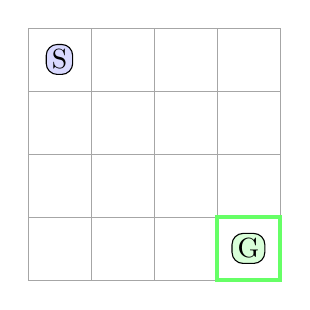
\begin{tikzpicture}[scale=0.8]
  % 4x4 grid
  \draw[step=1cm,gray!70,very thin] (0,0) grid (4,4);

  % Coordinates labels (optional, subtle)
  \foreach \x in {0,...,3} {
    \foreach \y in {0,...,3} {
      % Display convention: (0,0) is top-left, (3,3) is bottom-right
      %\node[gray!60,scale=0.6] at (\x+0.5,\y+0.5) {$(\y,\x)$};
    }
  }

  % Start and Goal
  \node[draw,rounded corners,fill=blue!15,inner sep=2pt] at (0.5,3.5) {S};
  \node[draw,rounded corners,fill=green!15,inner sep=2pt] at (3.5,0.5) {G};

  % Terminal border highlight
  \draw[very thick,green!60] (3,0) rectangle (4,1);
\end{tikzpicture}
\end{center}
}

\begin{document}

%------------------------------------------------
\begin{frame}
  \titlepage
  \note{Set expectations: we will use one GridWorld example to define all core RL objects and derive Bellman equations, then connect directly to Q-learning.}
\end{frame}

%------------------------------------------------
\begin{frame}{Outline}
  \tableofcontents
  \note{Emphasize the flow: environment model (MDP) -> interaction (episodes) -> behavior (policy) -> evaluation (values) -> recursion (Bellman) -> learning (Q-learning).}
\end{frame}

%------------------------------------------------
\section{Running Example: GridWorld}

\begin{frame}{Our Single Example: GridWorld}
\GridWorldFigure

\begin{itemize}
  \item State $s$ is the agent position on the grid
  \item Actions: $\mathcal{A} = \{\uparrow,\downarrow,\leftarrow,\rightarrow\}$
  \item Start at \textbf{S}, goal at \textbf{G} (terminal)
\end{itemize}

\note{Tell students: everything today will refer back to this picture. Avoid switching environments/examples.}
\end{frame}

\begin{frame}{GridWorld Dynamics and Rewards}
\begin{itemize}
  \item Deterministic transitions (most of the time):
  \begin{itemize}
    \item If an action would leave the grid, the agent stays in place
    \item Otherwise it moves one cell in the chosen direction
  \end{itemize}
  
  \vspace{0,3cm}
  
  \item Reward design (simple and common):
  \[
    R_{t+1} = -1 \text{ for each step until reaching } G
  \]
  \item Episode ends when the agent reaches $G$
\end{itemize}

\note{This reward makes shorter paths better. Mention that reward is part of the problem specification, not a property of the algorithm.}
\end{frame}

%------------------------------------------------
\section{Markov Decision Processes (MDPs)}

\begin{frame}{Markov Property}
A process is \textbf{Markov} if the future depends only on the present.

%\[
%\Pr(S_{t+1}=s' \mid S_t=s, A_t=a, S_{t-1},A_{t-1},\dots) = \Pr(S_{t+1}=s' \mid S_t=s, A_t=a)
%\]

\vspace{6pt}
In GridWorld:
\begin{itemize}
  \item Knowing the current cell and the chosen move is enough to predict the next cell
\end{itemize}

\note{Tie directly to intuition: memoryless dynamics once state is defined well enough.}
\end{frame}

\begin{frame}{Definition: Markov Decision Process}
An \textbf{MDP} is typically defined by:
\[
\langle \mathcal{S}, \mathcal{A}, p, r, \gamma \rangle
\]
\begin{itemize}
  \item $\mathcal{S}$: set of states
  \item $\mathcal{A}$: set of actions
  \item $p(s',r\mid s,a)$: dynamics + reward distribution
  \item $\gamma \in [0,1)$: discount factor
\end{itemize}

\vspace{6pt}
In GridWorld, $\mathcal{S}$ are grid cells and $p$ is deterministic.
\end{frame}

%------------------------------------------------
\section{Episodes and Returns}

\begin{frame}{Episodes}
\begin{itemize}
  \item An \textbf{episode} is a finite sequence:
  \[
  S_0, A_0, R_1, S_1, A_1, R_2, \dots, S_T
  \]
  \item $S_T$ is a \textbf{terminal} state (absorbing, end of interaction)
  \item GridWorld is \textbf{episodic}: each run ends when we reach the goal
\end{itemize}

\note{Contrast briefly with continuing tasks (e.g., thermostat control). For today, we stay episodic.}
\end{frame}

\begin{frame}{Return (What We Want to Maximize)}
The \textbf{return} from time $t$ is the discounted sum of future rewards:
\[
G_t = \sum_{k=0}^{T-t-1} \gamma^k R_{t+k+1}
\]

\vspace{6pt}
In GridWorld with $R=-1$ per step:
\begin{itemize}
  \item Larger return means fewer steps to reach $G$
  \item Discount $\gamma$ controls how much we care about near vs far future
\end{itemize}
\end{frame}


\begin{frame}{Why Discounting?}
Discounting ($\gamma \in [0,1)$) is mainly used to make returns well-defined and to express preference for sooner rewards.

\vspace{3pt}

\textbf{1) Infinite-horizon tasks can diverge without discounting}
\begin{itemize}
  \item In a continuing task (e.g., thermostat control), there may be no terminal time $T$.
  \item If rewards do not go to zero, the undiscounted sum can blow up:
  \[
    \sum_{k=0}^{\infty} R_{t+k+1} \quad \text{may diverge.}
  \]
\end{itemize}

\vspace{3pt}

\textbf{2) Interpreting $\gamma$}
\begin{itemize}
  \item Smaller $\gamma$: more short-term / myopic behavior
  \item Larger $\gamma$: more long-term planning (but still finite when $\gamma<1$)
\end{itemize}

\note{Emphasize the practical reason: in continuing problems, discounting makes the objective finite. Also mention the intuition: $\gamma$ controls how far into the future rewards matter.}
\end{frame}

%------------------------------------------------
\section{Policies}

\begin{frame}{Policies (Behavior)}
A \textbf{policy} $\pi$ specifies how the agent acts:
\[
\pi(a\mid s) = \Pr(A_t=a \mid S_t=s)
\]

\vspace{6pt}
Examples in GridWorld:
\begin{itemize}
  \item Random policy: choose each move with probability $1/4$
  \item Greedy-to-goal: prefer actions that reduce distance to $G$
\end{itemize}

\note{Highlight: a policy can be stochastic and still be optimal in some problems (not necessarily here).}
\end{frame}

%------------------------------------------------
\section{Value Functions}

\begin{frame}{State-Value Function $v_\pi$}
	
\textbf{The value of a state under policy $\pi$} is the expected return:

\[
 v_\pi(s) = \mathbb{E}_\pi\big[ G_t \mid S_t=s \big]
\]

Remember: 

\[
G_t = \sum_{k=0}^{T-t-1} \gamma^k R_{t+k+1}
\]

\vspace{6pt}
Interpretation in GridWorld:
\begin{itemize}
  \item How good is it to be in cell $s$ if we keep following $\pi$?
\end{itemize}
\end{frame}

\begin{frame}{Bellman Expectation Equation (State Values)}
	The value of a state decomposes into:
	\[
	v_\pi(s) = \sum_{a} \pi(a\mid s) \sum_{s',r} p(s',r\mid s,a)\,\big[r + \gamma v_\pi(s')\big]
	\]

\vspace{3pt}

\textbf{More intuitively:}

\begin{itemize}
	\item From state $s$, the policy chooses actions with probability $\pi(a \mid s)$.
	
	\item Each action can lead to different next states $s'$ and rewards $r$ with probability $p(s', r \mid s, a)$.
	
	\item For each possible outcome, you receive:
	\[
	\text{immediate reward} + \gamma \times \text{future value}
	\]
	
	\item You then take the weighted average of all these possibilities.
\end{itemize}

\end{frame}


\begin{frame}{Action-Value Function $q_\pi$}
The value of taking action $a$ in state $s$, following $\pi$:
\[
 q_\pi(s,a) = \mathbb{E}_\pi\big[ G_t \mid S_t=s, A_t=a \big]
\]

Remember: 

\[
G_t = \sum_{k=0}^{T-t-1} \gamma^k R_{t+k+1}
\]

\end{frame}




\begin{frame}{Bellman Expectation Equation (Action Values)}
Similarly for action values:
\[
 q_\pi(s,a) = \sum_{s',r} p(s',r\mid s,a)\,\Big[r + \gamma \sum_{a'} \pi(a'\mid s') q_\pi(s',a')\Big]
\]

More intuitively:

\begin{itemize}
	\item You start in $s$ and \emph{force action} $a$.
	\item The environment moves to some $s'$ and gives reward $r$ with probability $p(s', r \mid s, a)$.
	\item After arriving in $s'$, you follow the policy $\pi$, which chooses the next action $a'$.
	\item The future value is therefore the average $q_\pi(s', a')$ under $\pi$.
\end{itemize}

%\vspace{6pt}
%This is the key recursion behind many algorithms (DP, TD, Q-learning).
\end{frame}

%\begin{frame}{Optimal Value Functions}
%Define the best achievable values:
%\[
% v_*(s) = \max_\pi v_\pi(s), \qquad q_*(s,a) = \max_\pi q_\pi(s,a)
%\]
%
%\vspace{6pt}
%A policy $\pi_*$ is \textbf{optimal} if it achieves $v_*(s)$ for all states.
%\end{frame}

\begin{frame}{Bellman Optimality Equations}
State values:
\[
v_*(s) = \max_\pi v_\pi(s)
\]
\[
v_*(s) = \max_a \sum_{s',r} p(s',r\mid s,a)\,\big[r + \gamma v_*(s')\big]
\]

Action values:
\[
q_*(s,a) = \max_\pi q_\pi(s,a)
\]
\[
 q_*(s,a) = \sum_{s',r} p(s',r\mid s,a)\,\Big[r + \gamma \max_{a'} q_*(s',a')\Big]
\]

\note{Emphasize: the only change vs expectation equations is replacing policy averaging by max (control).}
\end{frame}

%------------------------------------------------
\section{Bridge to Q-Learning (Next Class)}

\begin{frame}{From Bellman Optimality to Learning}
If we knew $p(s',r\mid s,a)$, we could plan (Dynamic Programming).

\vspace{6pt}
In many real problems:
\begin{itemize}
  \item We \textbf{do not} know the dynamics model $p$
  \item We must learn from sampled transitions $(S_t,A_t,R_{t+1},S_{t+1})$
\end{itemize}

\vspace{6pt}
Next: \textbf{model-free control} with Q-learning.
\end{frame}

\begin{frame}{References}
\begin{itemize}
  \item Sutton, R. S., \& Barto, A. G. (2018). \textit{Reinforcement Learning: An Introduction}, 2nd ed. Chapter 3.
\end{itemize}
\end{frame}

\end{document}
